\documentclass[aspectratio=169]{beamer}

\usetheme{Madrid}
\usecolortheme{beaver}
\usepackage{listings}

\setbeamertemplate{navigation symbols}{}

\hypersetup{
    colorlinks=true,
    linkcolor=darkred,
    filecolor=magenta,      
    urlcolor=darkred,
    pdftitle={GHC's JavaScript Backend},
    % pdfpagemode=FullScreen,
    }

\lstset{
  showstringspaces=false,
  stringstyle=\ttfamily\color{red},
  commentstyle=\ttfamily,
  keywordstyle=
}

\AtBeginSection[]
{
  \begin{frame}
    \frametitle{Table of Contents}
    \tableofcontents[currentsection]
  \end{frame}
}

\title{GHC's JavaScript Backend}
\author{Sylvain HENRY}
\institute[IOG]{
\includegraphics[scale=0.2]{images/iohk-logo.png}}
\date[2023-06-09]{GHC Workshop\\7-9 June 2023}

\begin{document}

\frame{\titlepage}

%\begin{frame}
%\frametitle{Table of Contents}
%\tableofcontents
%\end{frame}

\begin{frame}
\frametitle{2023: Haskell in the browser}
\begin{itemize}
\item Two new backends arrived at once in GHC 9.6
\item WebAssembly backend
\begin{itemize}
\item Cf yesterday’s presentation by Cheng
\end{itemize}
\item JavaScript backend 
\begin{itemize}
\item This presentation
\end{itemize}
\end{itemize}
\end{frame}

\section{Motivation}


\begin{frame}
\frametitle{What Web backends bring to Haskell developers}
\begin{enumerate}
\item Front-end Web programming
\begin{itemize}
  \item Full-stack Haskell (cf Ryan Trinkle Lambda Jam 2018 talk on Youtube)
\end{itemize}
\item Standalone applications (portable, with a GUI)
\begin{itemize}
\item Node.JS engine bundled with HTML/CSS rendering engine
\item e.g. ElectronJS, NW.JS…
\end{itemize}
\end{enumerate}

\hspace{1cm}

\begin{itemize}
\item Two things that current Haskell ecosystem is bad at!
\begin{itemize}
\item Rated “immature” on the
\href{https://github.com/Gabriella439/post-rfc/blob/main/sotu.md}{State of Haskell Ecosystem} wiki page
\end{itemize}
\end{itemize}
\hspace{1cm}
\begin{itemize}
\item What’s really new: directly available from stock GHC
\begin{itemize}
\item Not from external projects such as GHCJS or Asterius
\end{itemize}
\end{itemize}
\end{frame}



\begin{frame}
\frametitle{ JS vs Wasm backend: do we really need both?}
\begin{center}

\includegraphics[scale=0.2]{images/js_vs_wasm.png}
\end{center}
\begin{itemize}
\item Different targets, different backend implementations, different trade-offs
\item JavaScript backend’s peculiarities
\begin{itemize}
\item Own Runtime System written in JavaScript
\item First GHC backend to target a managed platform
\item JavaScript easy to hack and to observe (debug)
\item GHCJS already proved that JavaScript can be used in production
\end{itemize}
\end{itemize}
\end{frame}


\begin{frame}
\frametitle{JS backend: a different RTS written in JavaScript}

\begin{columns}

\begin{column}{0.7\textwidth}
\resizebox{8cm}{!}
{
\begin{tabular}{ll}
\hline
\textbf{Backend or project} & \textbf{Runtime System (RTS)} \\ \hline
NCG, C, and LLVM backends & C \\
JS backend, GHCJS         & JS \\
Asterius                  & JS (not the same) \\
Wasm backend & C (compiled to Wasm) \\ \hline
\end{tabular}
}
\end{column}

\begin{column}{0.2\textwidth}

\includegraphics[scale=0.3]{images/queue_rts.png}
\end{column}
\end{columns}

\vspace{1cm}

\begin{itemize}
\item Full control of the toolchain
\begin{itemize}
\item The backend doesn’t rely on external tooling to convert from C to JS
\item We can have exactly the JS code we want
\item Analogous to native code generator (NCG) vs C/LLVM backends for codegen
  \begin{itemize}
    \item More work, but more control
  \end{itemize}
\end{itemize}
\item Demo: show rts/js
\end{itemize}
\end{frame}


\begin{frame}
\frametitle{JS backend: first to target a managed platform}
\begin{itemize}
\item "Managed platform": own heap, heap objects, and garbage collector
%\item Find bugs
%\begin{itemize}
%\item JS backend already found one bug (in some code generated by Alex)
%\item Simply because out-of-bound memory accesses raise exceptions in JS
%\item In the past, GHCJS similarly found bugs in the STM implementation
%\end{itemize}
\item Implies changes:
\begin{itemize}
\item No pointers
\begin{itemize}
\item Addr\# isn't represented with a number in JavaScript
\end{itemize}
\item Foreign heap objects need to be representable in Haskell codes
\begin{itemize}
  \item We probably need a new ManagedRef\# (aka JSVal\#) primitive type
\end{itemize}
\item C FFI imports should be avoided or avoidable
\begin{itemize}
\item E.g. by providing fallback Haskell code (e.g. ghc-bignum's native backend)
\end{itemize}
\end{itemize}
\item It will make implementing other backends easier
\begin{itemize}
\item E.g. JVM and CLR (.Net)
\end{itemize}
\end{itemize}
\end{frame}


\begin{frame}
\frametitle{JS backend: observability \& tinkering}

\begin{itemize}
\item Full control of the toolchain 
\begin{itemize}
\item No LLVM, wasi-sdk, assembler, linker…
\item No limitation due to external factors
\end{itemize}
\item JavaScript is interpreted and (quite) readable
\begin{itemize}
\item Observe and dump anything, even interactively
\item Useful for debugging
\end{itemize}
\item Many JavaScript tools available
\begin{itemize}
\item Profilers, debuggers...
\end{itemize}
\end{itemize}
\end{frame}


\begin{frame}
\frametitle{Demo: SumInt64}
\begin{enumerate}
\item Show sources
\item Build and run
\item Present artefacts
\item Load in Chromium perf debugger
\item Show STG
\item Primops
  \begin{itemize}
    \item subInt64\# in STG
    \item primops.txt.pp: Int64SubOp
    \item GHC.StgToJS.Prim: Int64SubOp
    \item rts/js/arith.js: h\$hs\_minusInt64
  \end{itemize}
\end{enumerate}
\end{frame}

\section{Relation to GHCJS}

\begin{frame}
\frametitle{GHCJS: overview}
\begin{itemize}
\item Independent project (github.com/ghcjs)
\item Haskell to JavaScript compiler
\item Supports full Haskell (threads, Template Haskell, finalizers…)
\begin{itemize}
\item Compared to alternatives like Fay or Haste
\end{itemize}
\item Developed since $\sim$2010
\item Used in production
\item Relies on a fork of GHC 8.x
\end{itemize}
\begin{center}
\alert{The JS backend reused code from GHCJS}
\end{center}
But why did we need the JS backend in the first place if we had GHCJS?
\end{frame}

\begin{frame}
\frametitle{GHCJS issues and JS backend current status}
GHCJS...
\begin{itemize}
\item[]

\includegraphics[height=1em]{images/check_green.png}
...is difficult to build (without Nix)

\item[]

\includegraphics[height=1em]{images/check_green.png}
...is stuck on old GHC

\item[]

\includegraphics[height=1em]{images/check_green.png}
...lacks CI

\item[]

\includegraphics[height=1em]{images/arrow-up-right-yellow.png}
...lacks documentation

\item[]

\includegraphics[height=1em]{images/arrow-up-right-yellow.png}
...is slow

\item[]

\includegraphics[height=1em]{images/arrow-up-right-yellow.png}
...lacks maintainers

\item[]

\includegraphics[height=1em]{images/arrow-down-right-red.svg.png}
...produces code that is too big

\end{itemize}
\end{frame}


\begin{frame}
\frametitle{Maintainers}
\begin{columns}

\begin{column}{0.6\textwidth}
GHCJS’ maintainers
\begin{itemize}
\item Victor Nazarov (2010)
\item Hamish Mackenzie (2011-2013)
\item Luite Stegeman (2012-2021)
\end{itemize}

JS backend’s maintainers
\begin{itemize}
\item Jeffrey Young
\item Josh Meredith
\item Luite Stegeman
\item Sylvain Henry
\item \textit{Add your name here}
\end{itemize}
\end{column}

\begin{column}{0.4\textwidth}
\begin{center}

\includegraphics[scale=0.3]{images/xkcd_2347.png}
\tiny\url{https://xkcd.com/2347/}
\end{center}
\end{column}

\end{columns}

\end{frame}


\begin{frame}[fragile]
\frametitle{Building GHC with the JS backend}
\begin{itemize}
\item Nearly identical to building native GHC
\item You need the Emscripten C to JS toolchain
\begin{itemize}
\item GHC requires a C toolchain
\item Used for configure script, platform constants (e.g.
  \texttt{sizeof(uint\_t)}), hsc2hs, CPP…
\end{itemize}
  \item \alert{Don't use \texttt{--freeze1} (doesn't work for cross-compilers)}
\end{itemize}

\vspace{1cm}

\texttt
{\footnotesize
\$ ./boot \\
\$ \alert{emconfigure} ./configure -{}-target=\alert{javascript-unknown-ghcjs} \\
\$ ./hadrian/build --flavour=default+no\_profiled\_libs+\alert{native\_bignum} -j \\
\vspace{0.5cm}
\textit{wait $\sim$30 minutes, depending on your hardware} \\
\vspace{0.5cm}
\$ alias ghc-js=`pwd`/\_build/stage1/bin/javascript-unknown-ghcjs-ghc\\
}
\end{frame}


\begin{frame}
\frametitle{Code size regression}
\begin{itemize}
\item We didn’t fully port GHCJS’ JS optimizer
\begin{itemize}
\item Reason: was slow and brittle; needed redesign and rewrite
\end{itemize}
\end{itemize}
\hspace{1cm}
\begin{center}
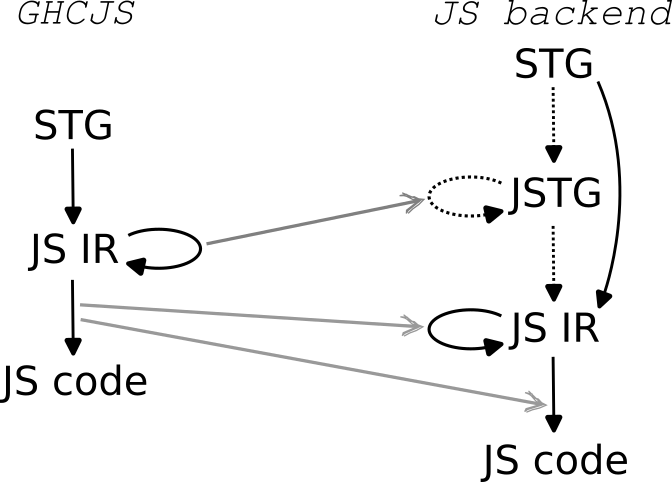
\includegraphics[scale=0.4]{images/pipelines.png}
\end{center}
\end{frame}



\begin{frame}
\frametitle{Key takeaways for GHCJS users}
\begin{itemize}
\item The JS backend is based on GHCJS but it isn’t GHCJS.
  \begin{itemize}
    \item Expect some changes
  \end{itemize}
\item GHCJS support is discontinued in favor of the JS backend.
\begin{itemize}
\item But it’s free software, anyone can pick it up
\end{itemize}
\item The JS backend isn't production-ready yet
\begin{itemize}
  \item Targeting GHC 9.10, cf roadmap (next topic)
\end{itemize}
\end{itemize}
\end{frame}

\section{Status \& Roadmap}

\begin{frame}
\frametitle{GHCJS upstreaming process(es)}

\begin{itemize}
\item Before 2022: make GHCJS converge towards GHC
\begin{itemize}
\item Avoid Template Haskell: e.g. replace JMacro QuasiQuoters
\item Only use boot libs: e.g. replace \texttt{lens}
\item Upgrade fork from GHC 8.6 to GHC 8.10
\end{itemize}

\item Since 2022: consider GHCJS as a prototype; implement a proper JS backend reusing GHCJS’ code
%\begin{itemize}
%\item Port code generator
%\item Port linker
%\item Setup CI for the JS backend (pass testsuite)
%\item Reuse GHC’s utilities: pretty-printer, binary serializer…
%\item Reimplement Template Haskell support
%\item … many other intermediate steps (500+ commits squashed into the initial commit)
%\end{itemize}
\end{itemize}
\end{frame}


\begin{frame}
\frametitle{Roadmap: GHC 9.6}
\begin{columns}

\begin{column}{0.3\textwidth}
\begin{center}

\includegraphics[height=5cm]{images/owl0.png}\\
1. Generate JS code from STG
\end{center}
\end{column}

\begin{column}{0.3\textwidth}
\begin{center}
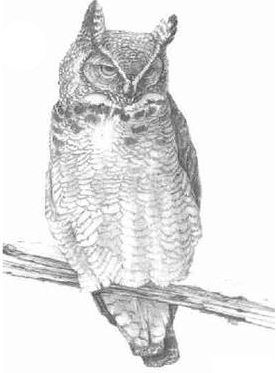
\includegraphics[height=5cm]{images/owl1.png}\\
2. Building working HelloWorld program
\end{center}
\end{column}

\begin{column}{0.3\textwidth}
\begin{center}
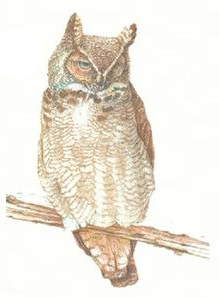
\includegraphics[height=5cm]{images/owl2.png}\\
3. Add CI,\\pass testsuite
\end{center}
\end{column}

\end{columns}
\end{frame}

\begin{frame}
\frametitle{Roadmap: GHC 9.8}
\begin{columns}

\begin{column}{0.3\textwidth}
\begin{center}
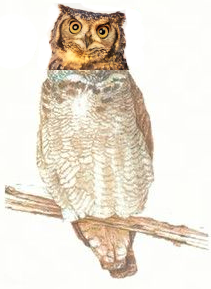
\includegraphics[height=4cm]{images/owl3.png}
\end{center}
\end{column}

\begin{column}{0.6\textwidth}
\begin{itemize}
\item FFI callbacks (see GHC Users' Guide)
\item Template Haskell (hopefully!)
\begin{itemize}
\item MR !9779
\end{itemize}
\end{itemize}
\end{column}

\end{columns}
\begin{center}

\includegraphics[height=2.3cm]{images/kmett.png}
\end{center}
\end{frame}


\begin{frame}
\frametitle{Roadmap: GHC 9.10+}
\begin{columns}

\begin{column}{0.25\textwidth}
\begin{center}
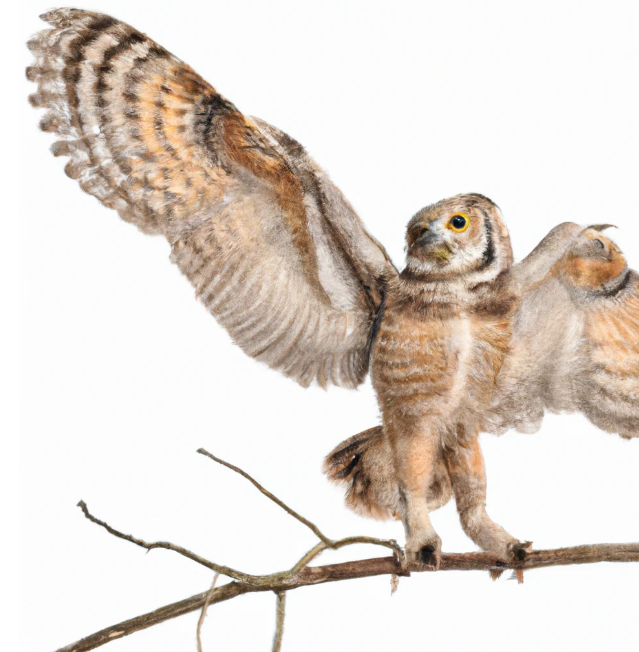
\includegraphics[width=3cm]{images/owl4.png}\\
\tiny Owl lift-off, via Dall-E
\end{center}
\end{column}

\begin{column}{0.7\textwidth}
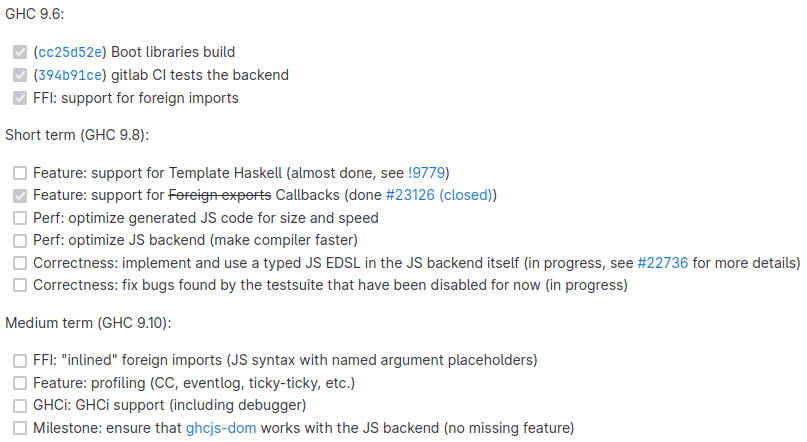
\includegraphics[height=6cm]{images/roadmap.png}
\end{column}

\end{columns}

\begin{center}
\url{https://gitlab.haskell.org/ghc/ghc/-/wikis/JavaScript-backend\#roadmap}
\end{center}

\end{frame}



\begin{frame}
\frametitle{GHCJS libraries need to be updated}

\begin{itemize}
\item GHCJS had a huge ecosystem
\item Initial plan: demo with some GHCJS' GUI framework (e.g. shine)
\item Not possible yet because packages need to be updated
\begin{itemize}
\item ghcjs-base, ghcjs-dom, jsaddle-*...
\item Adapt from GHC 8.x to GHC 9.x
\item Need to fix almost all FFI calls (next slide)
\end{itemize}
\end{itemize}
\end{frame}

%\begin{frame}[fragile]
%\frametitle{JavaScript FFI}
%
%\begin{lstlisting}[language=haskell]
%-- pre existing function
%foreign import javascript
%    "console.log"
%    js_log :: Int# -> Word# -> IO ()
%
%-- anonymous function
%foreign import javascript
%    "((x) => { console.log(x); })"
%    js_log :: Int# -> IO ()
%
%-- interruptible: explicit continuation
%foreign import javascript interruptible
%    "((x,c) => { c(x + 123); })"
%    js_foo :: Int# -> Int#
%\end{lstlisting}
%
%\end{frame}


\begin{frame}[fragile]
\frametitle{JavaScript FFI: GHCJS inline syntax is not supported}

\begin{lstlisting}[language=haskell]
-- GHCJS inline syntax: not supported!
foreign import javascript
    "$1===$2"
    js_eq :: JSString -> JSString -> Bool

-- replace with:
foreign import javascript
    "((x,y) => { return x===y; })"
    js_eq :: JSString -> JSString -> Bool

\end{lstlisting}

  \begin{itemize}
    \item Reasons
      \begin{itemize}
        \item need to add a JS parser to GHC
        \item need to coordinate with Wasm backend
        \item need a GHC proposal
      \end{itemize}
    \item In the meantime, please help updating GHCJS' libraries!
  \end{itemize}

\end{frame}

\begin{frame}
\frametitle{Demo: Svg}
  \begin{enumerate}
    \item Build and run with native backend
    \item Build and run with JS backend
      \begin{itemize}
        \item Show how to run cabal (build.sh)
        \item Run and debug
        \item js-sources (+bug)
      \end{itemize}
    \item Load in the browser
  \end{enumerate}
\end{frame}

%\begin{frame}[fragile]
%  \frametitle{JavaScript FFI: multi-variables values}
%  \begin{itemize}
%    \item Unboxed tuples, 64-bit types, Addr\#, etc. can’t be passed as a single JS value
%      \begin{itemize}
%    \item Passed as several arguments
%    \item Returned in additional h\$retN registers
%      \end{itemize}
%    \item Demo: FFI example
%  \end{itemize}
%
%\end{frame}


\section{Internals}



\begin{frame}
\frametitle{Execution model}
  \begin{itemize}
    \item Lazy graph reduction: STG machine in JavaScript
      \begin{itemize}
    \item Registers → JS global variables
    \item Stack → JS array
    \item Heap objects  → JS values (no storage manager in the JS RTS!)
      \end{itemize}
    \item Demo: present preamble of rts.js
      \begin{itemize}
        \item Registers
        \item Stack, sp
      \end{itemize}
    \end{itemize}
\end{frame}

\begin{frame}
\frametitle{Heap objects}
  \begin{itemize}
    \item STG objects: CONSTR, FUN, THUNK, PAP, BLACKHOLE…
      \begin{itemize}
        \item Represented in JS as object: \texttt{\{ f, d1, d2, m \}}
        \item f: properties ("info-table") and entry
          function
        \item d1, d2: payload
        \item m: mark used for heap traversal (weak references)
      \end{itemize}
    \item Demo: Constructors
      \begin{itemize}
        \item \texttt{-ddisable-js-minifier}
        \item Without optimization
        \item Present HS, STG and JS
        \item \texttt{h\$log(h\$mainZCMainzijust5);}
        \item \texttt{dumpCAF}
      \end{itemize}
  \end{itemize}
\end{frame}


\begin{frame}
  \frametitle{Mapping of primitive types}
  \begin{tabular}{ll}
    \hline
    Haskell & JavaScript \\ \hline
    Int\#, Word\#, Int8\#... & Number \\
    Float\#, Double\#        & Number\\
    Int64\#, Word64\#        & Two numbers (high, low) \\
    ByteArray\#...           & ArrayBuffer\\
    Array\#...               & Array\\
    MVar\#, ThreadID\#, Weak\#... & Object\\
    Addr\#                   & \alert{ArrayBuffer and number (offset)}\\
  \end{tabular}
  \hspace{1cm}
  \begin{itemize}
    \item Demo: Prim
      \begin{itemize}
        \item Show JS: \texttt{bar} returning primitive values
        \item Run: 2 mallocs with same "address" result
        \item Enable JS dump
      \end{itemize}
  \end{itemize}
\end{frame}


\begin{frame}
\frametitle{Scheduler}
  \begin{itemize}
    \item STG machine usually implemented with tail calls / goto
      \begin{itemize}
        \item JS engines don't support tail calls
        \item Using normal calls to implement tail calls would blow the JS call
          stack
      \end{itemize}

    \item What the JS backend does:
      \begin{itemize}
        \item Haskell functions are represented as 0-argument JS functions
          \begin{itemize}
            \item Arguments are passed via global variables
          \end{itemize}
        \item They \alert{return} their own continuation
        \item Trampoline in the scheduler: \texttt{while(true) \{ c = c(); \}}
      \end{itemize}
    \item Demo:
      \begin{itemize}
        \item show rts/js/thread.js runThreadSlice
        \item "Fun" demo (without optimizations)
        \item Show STG and JS for add10
        \item add a bang to x in add10
        \item add \texttt{h\$log(c.name)}
        \item add \texttt{if (c.name.match("main"))}
      \end{itemize}
        \item
          \url{https://engineering.iog.io/2023-04-21-stacks-in-the-js-backend}
  \end{itemize}
\end{frame}

\begin{frame}
\frametitle{Template Haskell interpreter}
  \begin{itemize}
    \item GHCJS pioneered the “external interpreter” idea
      \begin{itemize}
        \item Now we can reuse the upstream one!
      \end{itemize}
    \item Overview
      \begin{itemize}
    \item Execute js-interp.hs in Node.js
    \item Communicate via Unix pipes with it
    \item Can send compiled Haskell code to load and to execute
    \item First send the external interpreter code
    \item Then send TH splices and their dependencies
      \end{itemize}
  \end{itemize}
\end{frame}

\begin{frame}
  \frametitle{How to implement a new GHC backend: code overview}
  \begin{itemize}
\item Declare platform: ghc-boot:GHC.Platform.ArchOS
\item Fix build system: config.sub, hadrian, Cabal (js-sources),
  utils/deriveConstants
\item Add new IR: GHC.JS.Syntax
\item Add compilation pipeline: GHC.StgToJS.CodeGen
\item Add FFI support: GHC.HsToCore.Foreign.JavaScript
\item Fix boot libraries
  \begin{itemize}
\item JS: implement primitives (Posix…) using JS APIs
\item e.g. libraries/base/jsbits, js-sources, foreign import javascript
  \end{itemize}
\item Add linker support: GHC.StgToJS.Linker
\item Add runtime system or reuse existing one: rts/js/*
\item Add interpreter for Template Haskell: GHC.Runtime.Interpreter.JS and
  \texttt{js-interp.js}
\item Hook all this into the compiler driver: GHC.Driver.\{Backend...\}
\end{itemize}
\end{frame}


\section{Conclusion}

\begin{frame}
\frametitle{Contribution ideas}
  \begin{itemize}
   \item Build cool stuff with it and report/fix the issues you face!
   \item Help updating the GHCJS ecosystem and other libs (C sources...)
   \item Profile generated code and fix performance issues
    \begin{itemize}
   \item E.g. replace use of BigInt from numerical primop implementation
    \end{itemize}
   \item Help with any other item on the roadmap
     \begin{itemize}
   \item Fix skipped tests in the testsuite (grep "js\_broken")
   \item Profile GHC using the JS backend and optimize it
   \item (Re)implement support for profiling (cost centers...)
   \item Add JS code optimizations
   \item Fix \href{https://gitlab.haskell.org/ghc/ghc/-/issues?label\_name=javascript}{tickets with JavaScript label}
     \end{itemize}
   \item Support generating TypeScript code
   \item Support generating JS source maps
   \item Implement support for delimited continuation primops
   \item Your ideas here...
   \end{itemize}
\end{frame}


\begin{frame}
\frametitle{Contact}
  \begin{itemize}
    \item For assistance:
      \begin{itemize}
        \item Open tickets on GHC's gitlab
        \item ghc-devs mailing list
        \item sylvain.henry@iohk.io or sylvain@haskus.fr
      \end{itemize}
  \end{itemize}
  \vspace{2cm}
  \begin{center}
  Work funded by IOG\\
\includegraphics[scale=0.3]{images/iohk-logo.png}
  \end{center}
\end{frame}

\appendix

\section*{Appendix}

\begin{frame}[noframenumbering]
  \frametitle{Appendix}
\end{frame}

\begin{frame}[noframenumbering]
\frametitle{Potential IOG use cases}
\begin{itemize}
\item Code reuse
\begin{itemize}
\item Cardano blockchain network nodes written in Haskell
\item Reuse code to implement clients accessing the network
\item e.g. standalone GUI wallets, Web wallets
\end{itemize}
\item Full-stack Haskell for smart contracts
\begin{itemize}
\item Smart contracts fully written in Haskell
\item One part compiled to blockchain IR
\item Other part compiled to JS/Wasm to run into users’ wallets (UI)
\end{itemize}
\end{itemize}
\end{frame}

\end{document}
